\documentclass{if-beamer}

% --------------------------------------------------- %
%                  Presentation info	              %
% --------------------------------------------------- %
\title[Lecture 2]{Lecture 2}
\subtitle{Computer memory and the binary number system}
\author{Instructor: Ashley Gannon}
\date{ISC3313 Fall 2021}
\logo{

\includegraphics[scale=0.08]{figures/FSULogo.png}
}
\subject{Presentation subject} % metadata

\graphicspath{{figures/}}
% --------------------------------------------------- %
%                    Title + Schedule                 %
% --------------------------------------------------- %

\begin{document}

\begin{frame}
  \titlepage
\end{frame}

\begin{frame}
\frametitle{Memory device}
A memory device is a nifty gadget that allows us to store and recall information. This device has more than one state.\\

\begin{figure}
	\center
	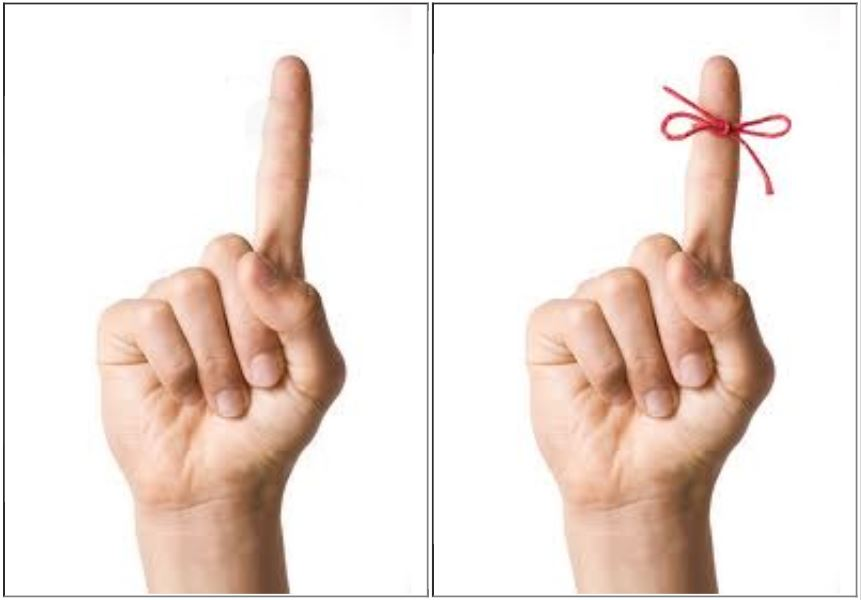
\includegraphics[width = 0.5\textwidth]{figures/finger.jpg}
\end{figure}
\end{frame}

\begin{frame}
\frametitle{Example}
Think of a light switch. It can either be on or off - one switch has 2 states. 

A row of n switches can be in $2^n$ states. For example, lets consider a row of 3 switches. 

\begin{figure}
	\center
	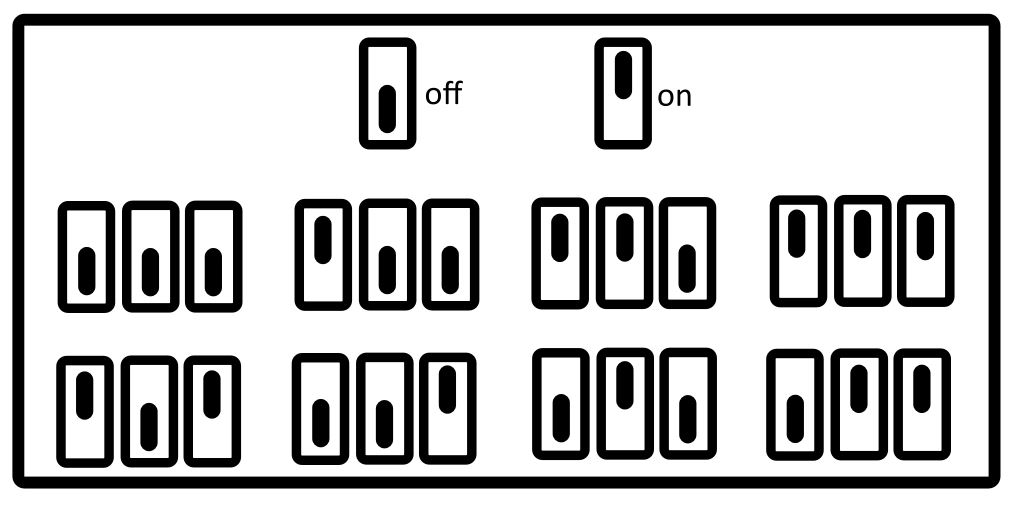
\includegraphics[width = 0.5\textwidth]{figures/lights.jpg}
\end{figure}

$2^3 = 8$ and we can see in this figure, there are $8$ possible states. We can number these possible states 0-7 and represent them using the binary number system.  

\end{frame}

\begin{frame}
\frametitle{Binary}
The binary number system, or base-two number system, uses 2 digits to encode a number - 0 or 1. \\~\

Let's compare base-two with base-ten. In base ten, decimal, you have columns for $10^0 = 1$ (ones), $10^1 = 10$ (tens), $10^2 = 100$ (hundreds), $10^3 = 1000$ (thousands), etc. In base two, you have columns for $2^0 = 1$ (ones), $2^1 = 2$ (twos), $2^2 = 4$ (fours), $2^3 = 8$ (eights) and so on. 

\begin{figure}
	\center
	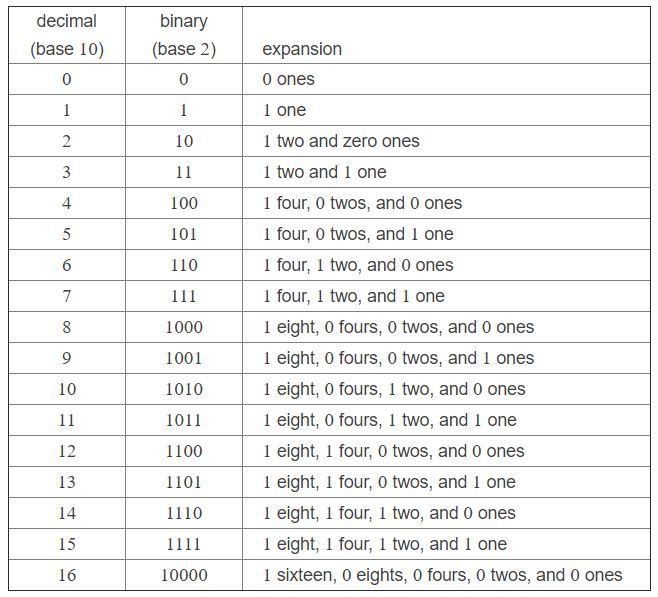
\includegraphics[width = 0.5\textwidth]{figures/table.jpg}
\end{figure}

\end{frame}

\begin{frame}
\frametitle{Light switch example}
Let's go back to our light switch example. I'll give you a few minutes to fill in the rest. NOTE: The only coefficients you may use are 0 or 1. 
\begin{figure}
	\flushleft
	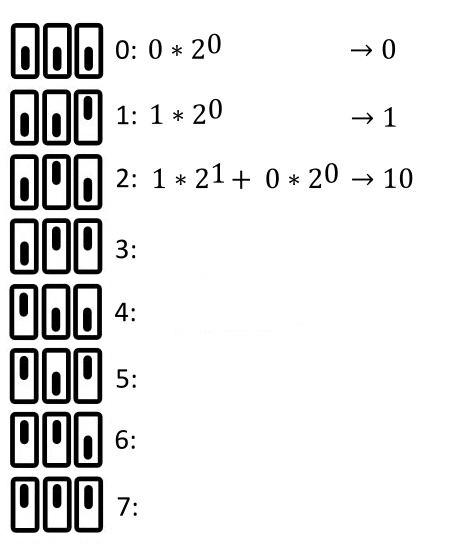
\includegraphics[width = 0.5\textwidth]{figures/fillinex.jpg}
\end{figure}
\end{frame}

\begin{frame}
\frametitle{Converting larger base ten numbers to base two numbers}

Obviously, the approach we used in the last example would be tedious to do on a larger number. \\~\

Let's convert $357_{10}$ to base two. An easy way to do this is to divide by 2, keeping track of the remainders as you go. \\~\
\end{frame}

\begin{frame}
\frametitle{Converting larger base ten numbers to base two numbers}

Obviously, the approach we used in the last example would be tedious to do on a larger number. Let's convert $357_{10}$ to base two. An easy way to do this is to divide by 2, keeping track of the remainders as you go. \\~\

\centering
\begin{align*}
357/2 &= 178 \textrm{R}\textbf{1} \\
\end{align*}
\end{frame}

\begin{frame}
\frametitle{Converting larger base ten numbers to base two numbers}

Obviously, the approach we used in the last example would be tedious to do on a larger number. Let's convert $357_{10}$ to base two. An easy way to do this is to divide by 2, keeping track of the remainders as you go. \\~\

\centering
\begin{align*}
357/2 &= 178 \textrm{R}\textbf{1} \\
178/2 &= 89 \textrm{R}\textbf{0}\\
\end{align*}
\end{frame}

\begin{frame}
\frametitle{Converting larger base ten numbers to base two numbers}

Obviously, the approach we used in the last example would be tedious to do on a larger number. Let's convert $357_{10}$ to base two. An easy way to do this is to divide by 2, keeping track of the remainders as you go. \\~\

\centering
\begin{align*}
357/2 &= 178 \textrm{R}\textbf{1} \\
178/2 &= 89 \textrm{R}\textbf{0}\\
89/2 &= 44 \textrm{R}\textbf{1}\\
\end{align*}
\end{frame}

\begin{frame}
\frametitle{Converting larger base ten numbers to base two numbers}

Obviously, the approach we used in the last example would be tedious to do on a larger number. Let's convert $357_{10}$ to base two. An easy way to do this is to divide by 2, keeping track of the remainders as you go. \\~\

\centering
\begin{align*}
357/2 &= 178 \textrm{R}\textbf{1} \\
178/2 &= 89 \textrm{R}\textbf{0}\\
89/2 &= 44 \textrm{R}\textbf{1}\\
44/2 &= 22 \textrm{R}\textbf{0}\\
\end{align*}
\end{frame}

\begin{frame}
\frametitle{Converting larger base ten numbers to base two numbers}

Obviously, the approach we used in the last example would be tedious to do on a larger number. Let's convert $357_{10}$ to base two. An easy way to do this is to divide by 2, keeping track of the remainders as you go. \\~\

\centering
\begin{align*}
357/2 &= 178 \textrm{R}\textbf{1} \\
178/2 &= 89 \textrm{R}\textbf{0}\\
89/2 &= 44 \textrm{R}\textbf{1}\\
44/2 &= 22 \textrm{R}\textbf{0}\\
22/2 &= 11 \textrm{R}\textbf{0}\\
\end{align*}
\end{frame}

\begin{frame}
\frametitle{Converting larger base ten numbers to base two numbers}

Obviously, the approach we used in the last example would be tedious to do on a larger number. Let's convert $357_{10}$ to base two. An easy way to do this is to divide by 2, keeping track of the remainders as you go. \\~\

\centering
\begin{align*}
357/2 &= 178 \textrm{R}\textbf{1} \\
178/2 &= 89 \textrm{R}\textbf{0}\\
89/2 &= 44 \textrm{R}\textbf{1}\\
44/2 &= 22 \textrm{R}\textbf{0}\\
22/2 &= 11 \textrm{R}\textbf{0}\\
11/2 &= 5 \textrm{R}\textbf{1}\\
\end{align*}
\end{frame}

\begin{frame}
\frametitle{Converting larger base ten numbers to base two numbers}

Obviously, the approach we used in the last example would be tedious to do on a larger number. Let's convert $357_{10}$ to base two. An easy way to do this is to divide by 2, keeping track of the remainders as you go. \\~\

\centering
\begin{align*}
357/2 &= 178 \textrm{R}\textbf{1} \\
178/2 &= 89 \textrm{R}\textbf{0}\\
89/2 &= 44 \textrm{R}\textbf{1}\\
44/2 &= 22 \textrm{R}\textbf{0}\\
22/2 &= 11 \textrm{R}\textbf{0}\\
11/2 &= 5 \textrm{R}\textbf{1}\\
5/2 &= 2 \textrm{R}\textbf{1}\\
\end{align*}
\end{frame}

\begin{frame}
\frametitle{Converting larger base ten numbers to base two numbers}

Obviously, the approach we used in the last example would be tedious to do on a larger number. Let's convert $357_{10}$ to base two. An easy way to do this is to divide by 2, keeping track of the remainders as you go. \\~\

\centering
\begin{align*}
357/2 &= 178 \textrm{R}\textbf{1} \\
178/2 &= 89 \textrm{R}\textbf{0}\\
89/2 &= 44 \textrm{R}\textbf{1}\\
44/2 &= 22 \textrm{R}\textbf{0}\\
22/2 &= 11 \textrm{R}\textbf{0}\\
11/2 &= 5 \textrm{R}\textbf{1}\\
5/2 &= 2 \textrm{R}\textbf{1}\\
2/2 &= \textbf{1}\textrm{R}\textbf{0} \\
\end{align*}
\end{frame}

\begin{frame}
\frametitle{Converting larger base ten numbers to base two numbers}

Obviously, the approach we used in the last example would be tedious to do on a larger number. Let's convert $357_{10}$ to base two. An easy way to do this is to divide by 2, keeping track of the remainders as you go. \\~\

\centering
\begin{align*}
357/2 &= 178 \textrm{R}\textbf{1} \\
178/2 &= 89 \textrm{R}\textbf{0}\\
89/2 &= 44 \textrm{R}\textbf{1}\\
44/2 &= 22 \textrm{R}\textbf{0}\\
22/2 &= 11 \textrm{R}\textbf{0}\\
11/2 &= 5 \textrm{R}\textbf{1}\\
5/2 &= 2 \textrm{R}\textbf{1}\\
2/2 &= \textbf{1}\textrm{R}\textbf{0} \\
\end{align*}

Now start with the last whole number and move up through the remainders. 
\centering
$375_{10} = 101100101_2$
\end{frame}

\begin{frame}
\frametitle{Converting larger base ten numbers to base two numbers}
Now let's check that this is correct: 
$375_{10} = 101100101_2$.
The first thing we want to do is number the digits of $101100101$from right to left - keep in mind the right-most digit is the remainder from the first divide.
\begin{figure}
	\centering
	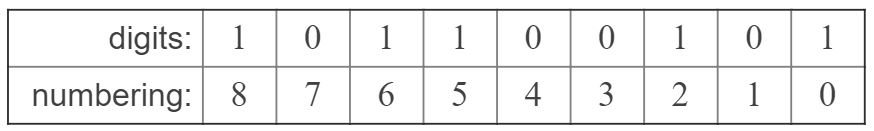
\includegraphics[width = 0.5\textwidth]{figures/digits.jpg}
\end{figure}
\end{frame}

\begin{frame}
\frametitle{Converting larger base ten numbers to base two numbers}
Now let's check that this is correct: 
$375_{10} = 101100101_2$.
The first thing we want to do is number the digits of $101100101$from right to left - keep in mind the right-most digit is the remainder from the first divide.
\begin{figure}
	\centering
	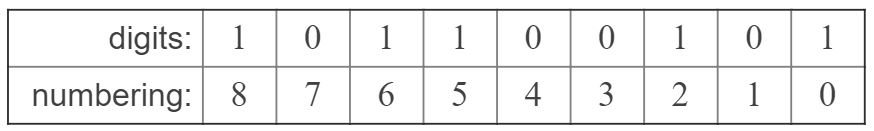
\includegraphics[width = 0.5\textwidth]{figures/digits.jpg}
\end{figure}
Now we can write out the series

$$101100101_2 = 1*2^8 + 0*2^7 + 1*2^6 + 1*2^5 + 0*2^4 + 0*2^3 + 1*2^2 + 0*2^1 + 1*2^0$$
\end{frame}

\begin{frame}
\frametitle{Converting larger base ten numbers to base two numbers}
Now let's check that this is correct: 
$357_{10} = 101100101_2$.
The first thing we want to do is number the digits of $101100101$ from right to left - keep in mind the right-most digit is the remainder from the first divide.
\begin{figure}
	\centering
	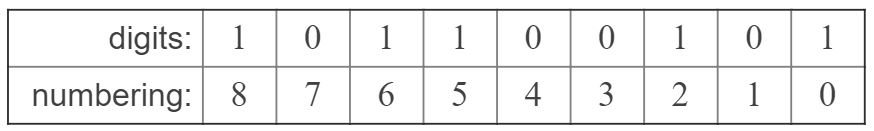
\includegraphics[width = 0.5\textwidth]{figures/digits.jpg}
\end{figure}
Now we can write out the series

$$101100101_2 = 1*2^8 + 0*2^7 + 1*2^6 + 1*2^5 + 0*2^4 + 0*2^3 + 1*2^2 + 0*2^1 + 1*2^0$$
$$101100101_2 = 256 + 0 + 64 + 32 + 0 + 0 + 4 + 0 + 1 = 357_{10}$$ 

\end{frame}

\begin{frame}
\frametitle{Class Activity}
\flushleft
Please determine how these base ten numbers would be written as base two numbers: \\~\

\begin{itemize}
	\setlength\itemsep{8em}
	\item $714_{10}$ \\
	\item $179_{10}$ \\
	\item $1428_{10}$ \\
	\item
\end{itemize}
\end{frame}

\begin{frame}
\frametitle{Class Activity}
Show the following are true: \\~\

\begin{itemize}
	\setlength\itemsep{8em}
	\item $1011001010_2 \rightarrow 714_{10}$
	\item $10110011_2 \rightarrow 179_{10}$
	\item $10110010100_2 \rightarrow 1428_{10}$
\end{itemize}
\end{frame}




% --------------------------------------------------- %
%                      Presentation                   %
% --------------------------------------------------- %

\end{document}
